% Chapter Template

\chapter{L'algoritmo H265} % Main chapter title

\label{Chapter4} % Change X to a consecutive number; for referencing this chapter elsewhere, use \ref{ChapterX}

\lhead{Capitolo 4. \emph{L'algoritmo H265}} % Change X to a consecutive number; this is for the header on each page - perhaps a shortened title

%----------------------------------------------------------------------------------------
%	SECTION 1
%----------------------------------------------------------------------------------------

\section{Suddivisione in blocchi dell'immagine} 
Un'immagine viene inizialmente suddivisa in \emph{coding tree unit} (CTU), di 
forma quadrata e dimensione costante per tutta la sequenza video: 64x64, 32x32 
o 16x16 pixel. Questa ``flessibilità'' nella dimensione del blocco fondamentale 
della suddivisione è stata introdotta da HEVC, in quanto tutti i suoi 
predecessori utilizzano un \emph{macroblocco} di 16x16 pixel; ciò permette a 
HEVC di sapersi adattare meglio a -e comprimere maggiormente- video di diverse 
dimensioni.
Il CTU è un'unità logica che consiste di tre ulteriori blocchi: Luma, 
ChromaB e ChromaR (Y, Cb e Cr). Ognuno di questi blocchi è un 
\emph{coding tree block} (CTB), ed è della stessa dimensione relativa 
del CTU, sebbene la dimensione effettiva di ogni blocco sia regolata dal 
\emph{chroma sampling format}: se il formato fosse 4:2:0, tipico di questi 
encoding, il blocco Y sarebbe 64x64 pixel, mentre i due blocchi di crominanza 
risulterebbero di 32x32 pixel. Quando un blocco risulta più piccolo del 
CTU di partenza (in questo caso, e quasi sempre, i due di crominanza) 
subisce un \emph{upscaling}: questo comporta una minore definizione e una 
maggiore compressione dell'immagine finale, resa ammissibile dalla maggiore 
sensibilità dell'apparato visivo umano alla luminanza rispetto al colore.
\begin{figure}[H]
  \centering
    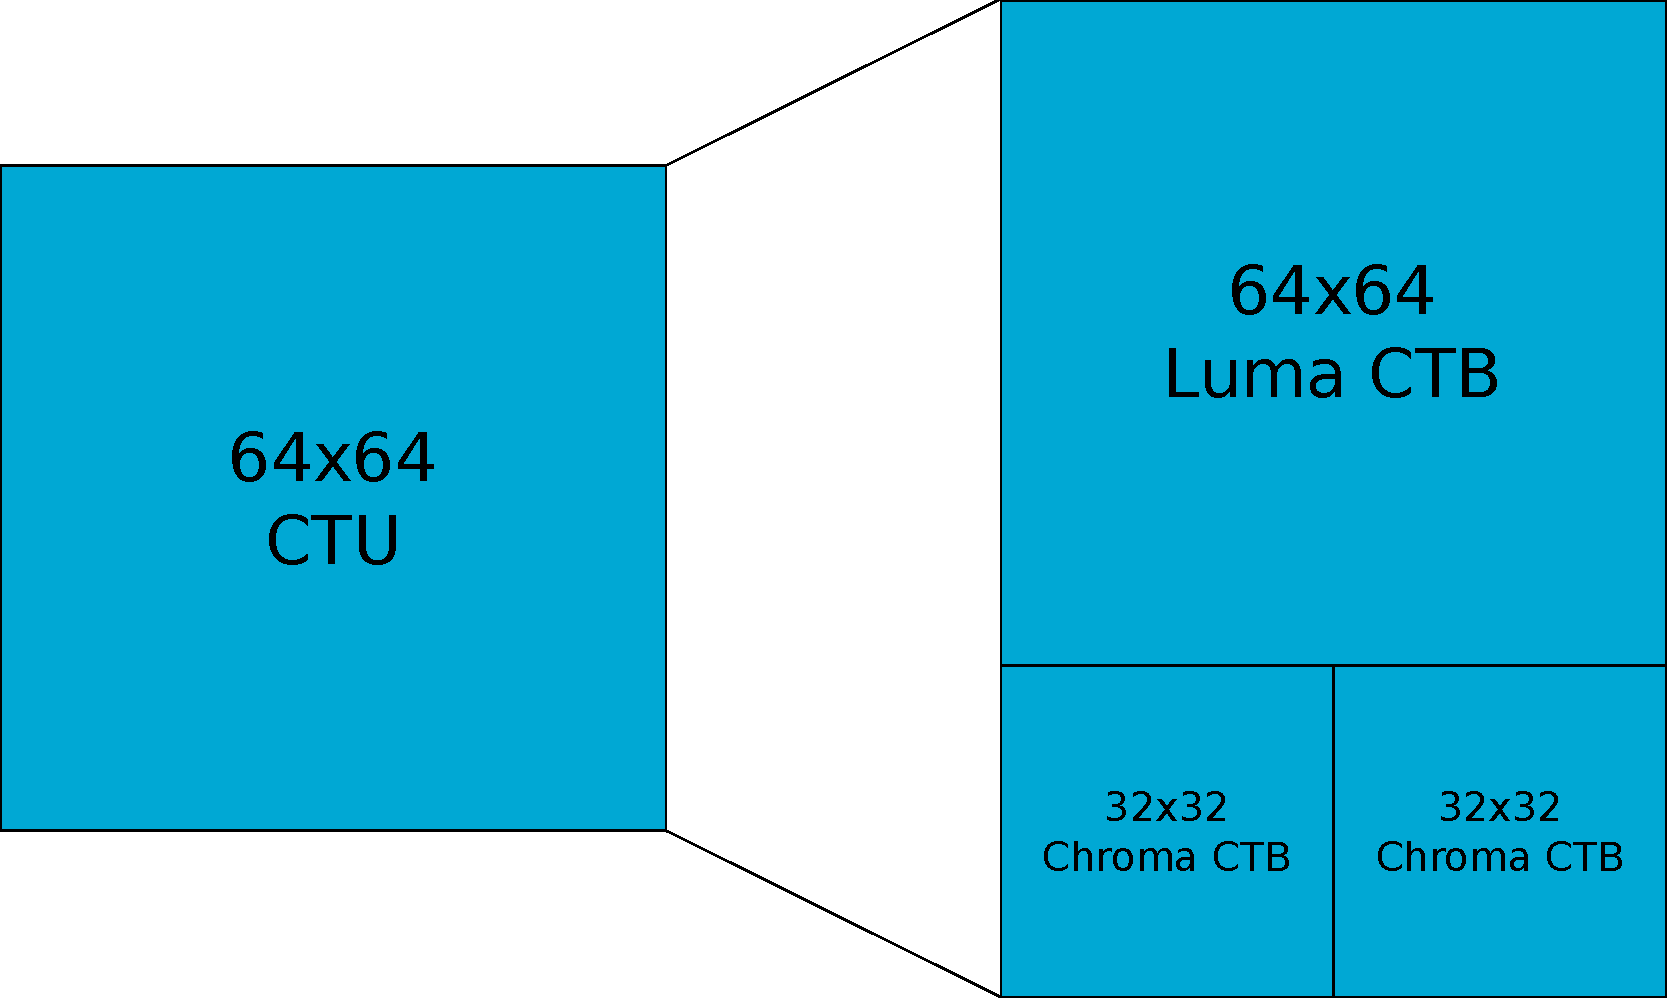
\includegraphics[scale=0.20]{Figures/CTU-CTB}
  \caption{Suddivisione del CTU in CTB}
\end{figure}
// Rivedere questo paragrafo: ovunque viene detto che il CTB è suddiviso \\
// in CU. \\
Il CTB può essere ulteriormente suddiviso in \emph{coding blocks} (CB), che 
sono il punto in cui viene decisa quale tipo di \emph{prediction} utilizzare.
Supponendo di avere un CTB di dimensione 64x64 la suddivisione può essere 
effettuata con CB grandi 64x64, 32x32, 16x16 o 8x8, ottenendo una struttura
detta \emph{quad-tree}, in cui il CTB è suddiviso ricorsivamente. 
Il CB, così come il CTB, consiste ancora nei tre blocchi Y, Cb e 
Cr, che definiscono un \emph{coding unit} (CU), ovverò l'unità in cui viene 
codificato il tipo di predizione. La scelta di quest'ultima è autonoma per ogni 
CU.
\begin{figure}[H]
  \centering
  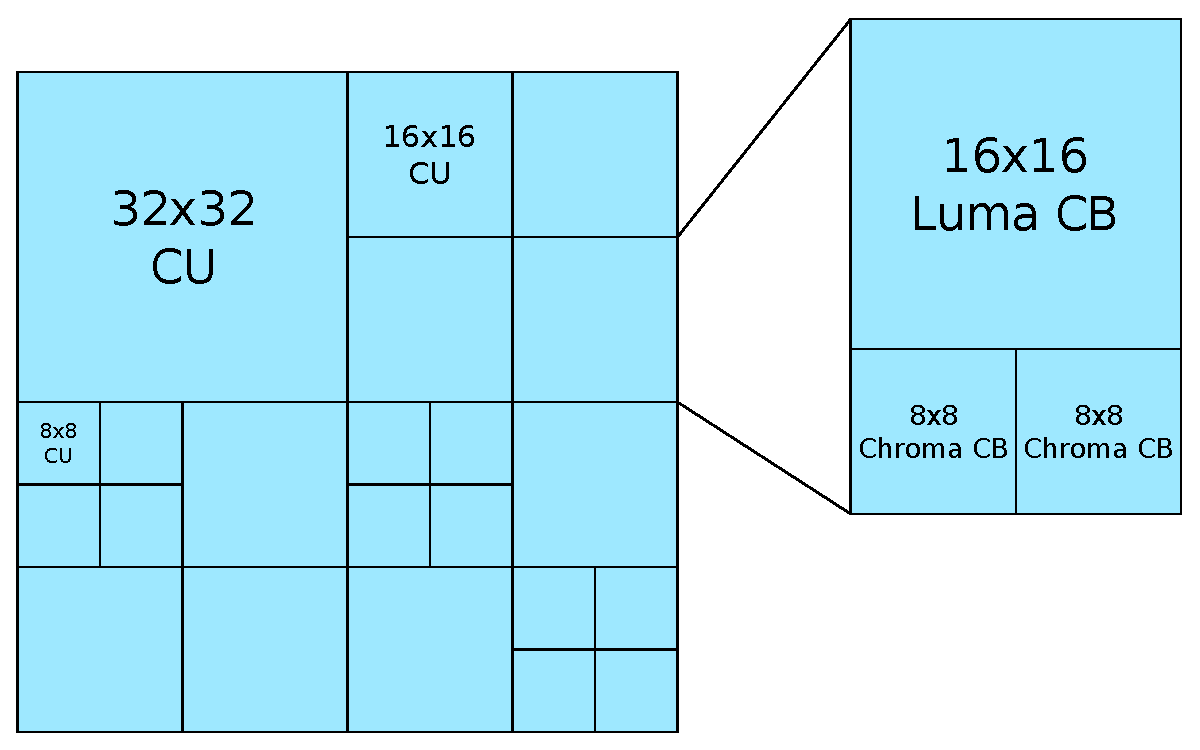
\includegraphics[scale=0.50]{Figures/CTB-CU-CB}
  \caption[Suddivisione del CTB in CU]{Suddivisione di un CTB 64x64 in una 
struttura a \emph{quadtree}}
\end{figure}
In caso ci sia bisogno di una maggiore precisione nella predizione (e.g., 
oggetti minuscoli che si muovono in un CB 8x8) è possibile suddividere i
\emph{coding block} in \emph{prediction block} (PB), che, in caso di 
\emph{inter prediction}, possono non seguire la struttura a \emph{quadtree} dei
blocchi precedenti:
\begin{figure}[H]
  \centering
  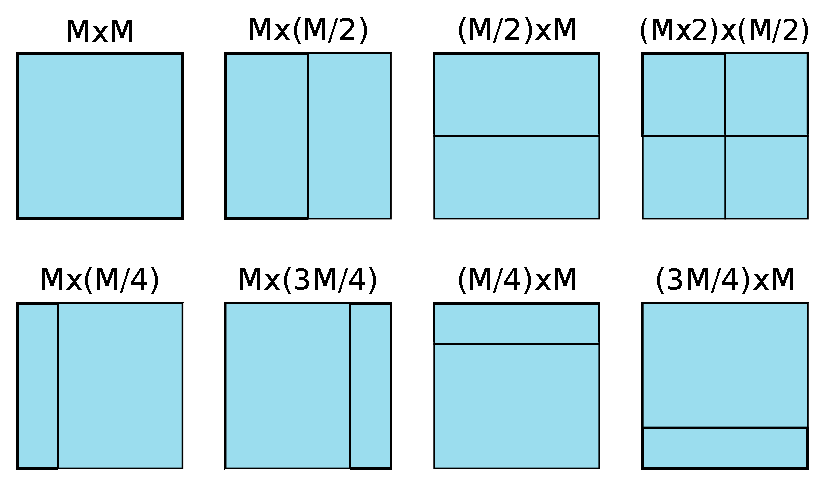
\includegraphics[scale=0.50]{Figures/PB}
  \caption{Possibili strutture di un \emph{prediction block}}
\end{figure}
Un PB definisce una regione che, per effettuare una predizione, utilizza gli 
stessi parametri di movimento: il numero di ipotesi di movimento (che può 
valere uno o due a seconda che si usi l'immagine precedente o quest'ultima 
e le successiva per cercare il blocco che si è mosso) e, per ognuna di queste, 
l'indice dell'immagine di riferimento e il vettore di movimento.
L'insieme dei tre PB, che possiedono lo stesso tipo di suddivisione, 
forma una \emph{prediction unit} (PU).
Per effettuare la codifica del segnale di errore un CB viene suddiviso in 
\emph{transform block}, dando forma ad una struttura a \emph{quadtree} che 
viene chiamata \emph{residual quadtree} (RQT); solitamente la suddivisione 
è mantenuta uguale per i TB Luma e Chroma.
%----------------------------------------------------------------------------------------
%	SECTION 2
%----------------------------------------------------------------------------------------

\section{Intra prediction}
Su un blocco di campioni contigui che possiedono gli stessi parametri 
predittivi, siano essi CB o PB, verrà eseguita la stessa 
\emph{intra prediction}.
Di quest'ultima esistono due tipologie a seconda delle caratteristiche 
del blocco: in caso di figure e strutture geometriche sarà utilizzata 
la \emph{angular prediction}, viceversa, se la predizione viene eseguita 
su contenuti meno strutturati, sarà eseguita una \emph{planar + DC prediction}. 
In entrambi i casi, la predizione si basa sui campioni contigui (o 
\emph{neighbour}) al blocco che si trovano a sinistra e a destra di 
quest'ultimo.

\paragraph*{Pre-filtering}
Prima di effettuare una delle due predizioni è possibile eseguire uno 
\emph{smoothing filter} sui campioni di riferimento, che dipende dal tipo di 
predizione che verrà successivamente eseguita. Le due possibilità sono le 
seguenti:
\begin{enumerate}
\item Un semplice \emph{lowpass filter} lineare con risposta all'impulso 
[1 2 1]/4 (a)
\item Se la dimensione del TB è 32x32 e i campioni di riferimento sono 
abbastanza ``morbidi'', questi vengono sostituiti con le corrispondenti 
interpolazioni lineari dei cambioni agli estremi (b)
\end{enumerate}

\begin{figure}[H]
  \centering
  \begin{tabular}{cc}
    \subfloat[]{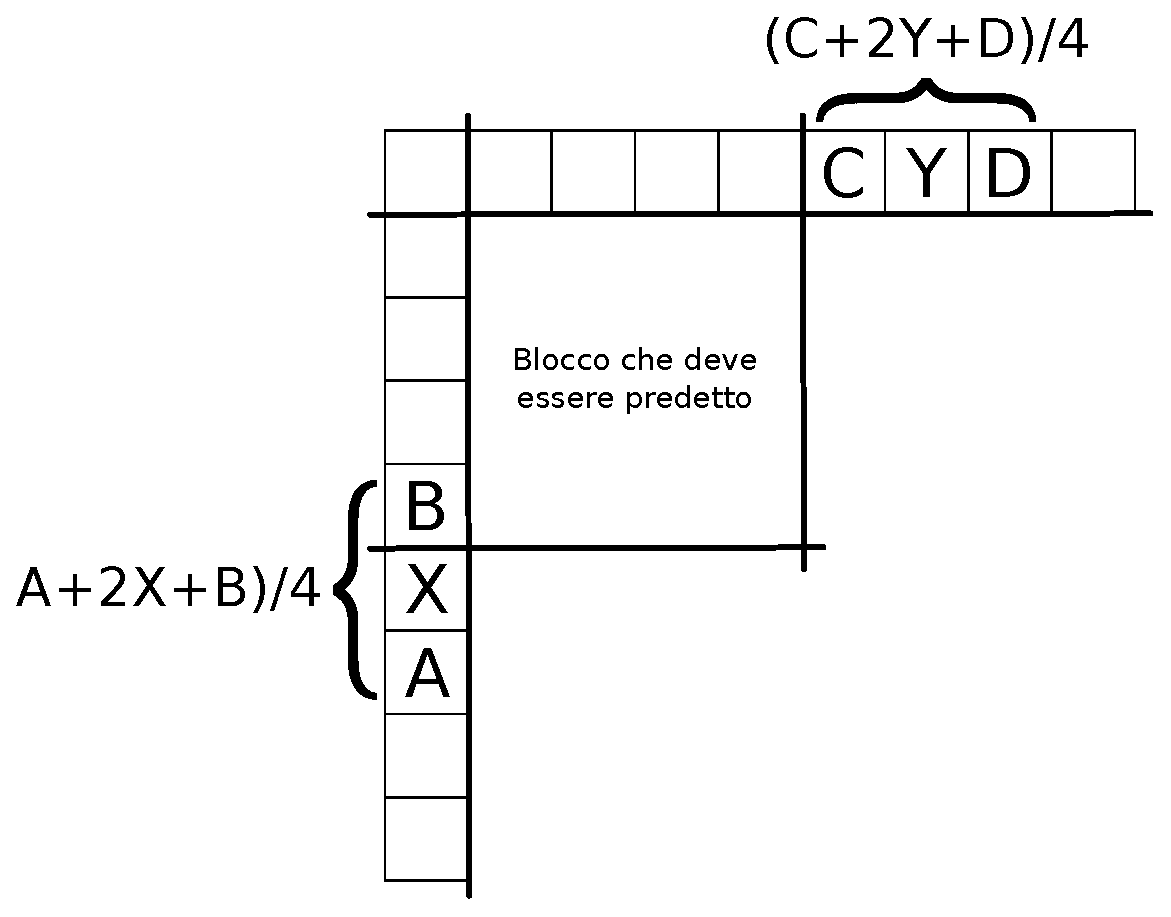
\includegraphics[scale=.35]{Figures/Filtering_a}}
    &
    \subfloat[]{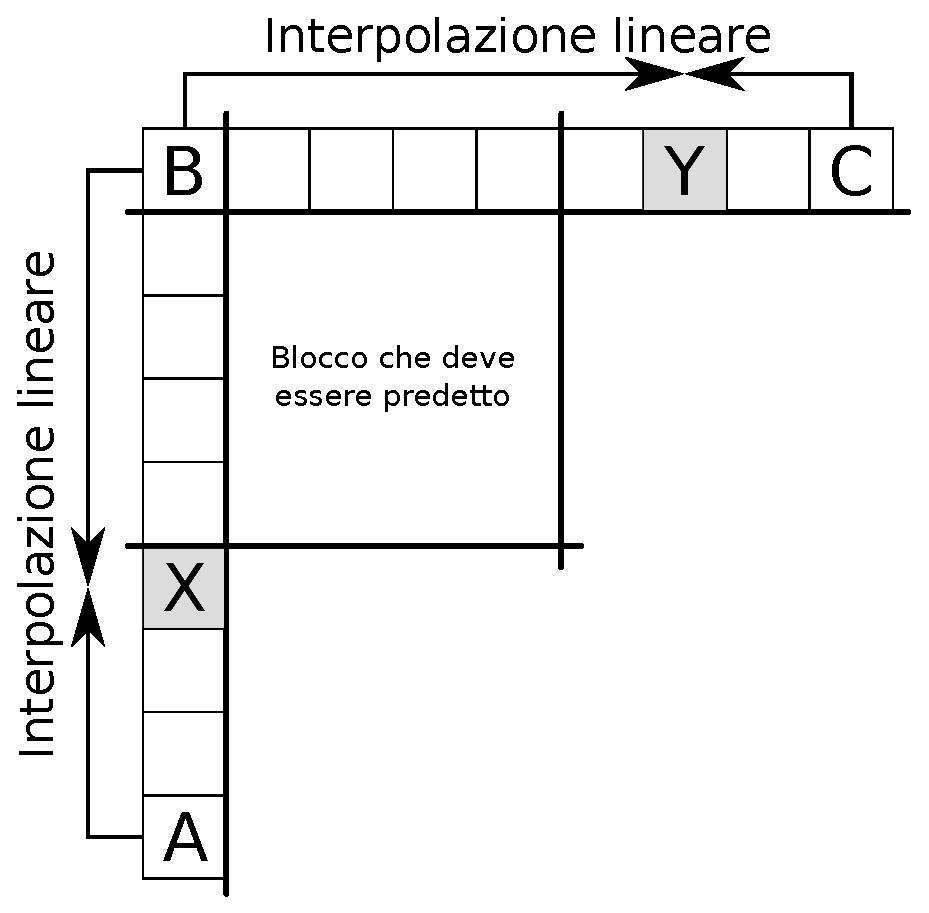
\includegraphics[scale=.35]{Figures/Filtering_b}}
  \end{tabular}
  \caption{I due diversi tipi di \emph{pre-filtering}}
\end{figure}
%-----------------------------------
%       SUBSECTION 1
%-----------------------------------

\subsection{Placeholder}

%-----------------------------------
%       SUBSECTION 2
%-----------------------------------

\subsection{Transform, Scaling \& Quantization}

%-----------------------------------
%       SUBSECTION 3
%-----------------------------------

\subsection{CABAC Entropy Coding}

%----------------------------------------------------------------------------------------
%       SECTION 3
%----------------------------------------------------------------------------------------

\section{Decoder}

%-----------------------------------
%       SUBSECTION 1
%-----------------------------------

\subsection{Intra Prediction}

%-----------------------------------
%       SUBSECTION 2
%-----------------------------------

\subsection{Inter Prediction}

%-----------------------------------
%       SUBSECTION 3
%-----------------------------------

\subsection{Scaling \& Inverse Transform}

%-----------------------------------
%       SUBSECTION 4
%-----------------------------------

\subsection{In-Loop Filter}

%-----------------------------------
%       SUBSECTION 5
%-----------------------------------

\subsection{DPB \& Output}
